 \chapter{Asynchronous programming. Node.js. Strategies and performance}
\section{Asynchronous programming}
Asynchronous programming is the programming model in which operations should be done are interleaved with one another within the single control thread. Analogy to it can be package multiplexing in a Computer Networks. 

To compare to multithreaded systems asynchorous allow execution of one task per unit of time. Further, tread suspension/invocation lays outside programmer's control while in asynchonous system task will run untill programmer will perform explicit control delegation to other task.\cite{asyncArticle} 

In contrast to synchronous systems where process can be blocked by one another (i. e. waiting response from I/O) asynchronous system instead of waiting will switch to execution of the next task in a thread.

Generally asynchronous systems are easier to control and to develop rather then multithreaded, and  they perfrom better then synchronous in following cases\cite{asyncArticle}:
 \begin{itemize}
	\item Large number of tasks and at least one task likely to make progress;
	\item A lot of I/O operations;
	\item Tasks are independent from one another;
 \end{itemize}

More detailed asynchronous system will be described in the end of the next section on an example of Node.js.

\section{Node.js}
Node.js is an asynchronous event driven framework designed to build scalable network applications.
Node.js is similar in design to and influenced by systems like Ruby's Event Machine or Python's Twisted with difference that it presents the event loop as a language construct instead of as a library\cite{nodejsabout}.

Node.js applications are written in JavaScript "a lightweight, interpreted, programming language with first-class functions. Most well-known as the scripting language for Web pages, many non-browser environments use it such as node.js and Apache CouchDB. JS is a prototype-based, multi-paradigm, dynamic scripting language, supporting object-oriented, imperative, and functional programming styles" as defined by Mozilla\cite{mozillaJS} which makes lowers entry border for the developers due to the language age and commonality.
 
npm ecosystem includes \textit{npm} - package manager for Node.js, \textit{npm Registry} - public collection of packages of open-source code, \textit{npm comand line clinet} which allows developers to install and publish those packages. On a diagram (\ref{fig:npmStat}) stated the comparison of npm with other package managers made by module counts, for more up to date information please visit \url{http://www.modulecounts.com/}
\begin{figure}[ht]
  	\label{fig:npmStat}
    \centering
    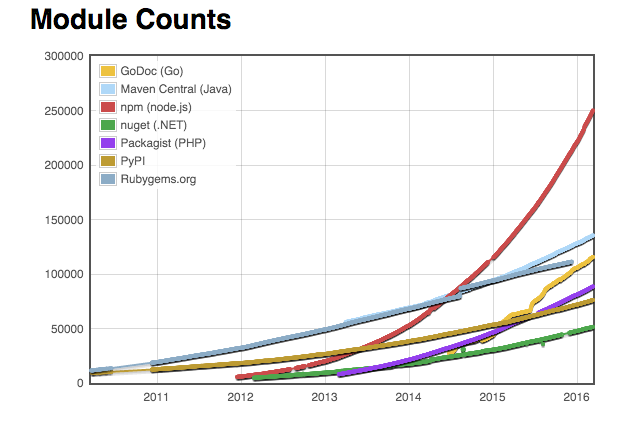
\includegraphics[width=\textwidth]{grafiken/modulecounts.png}
     \caption{npm comparison with other package managers\cite{moduleCounts}}
  \end{figure}

The highlevel architecture of Node.js looks following:(\ref{fig:nodeArch}). 
\begin{figure}[ht]
  	\label{fig:nodeArch}
    \centering
    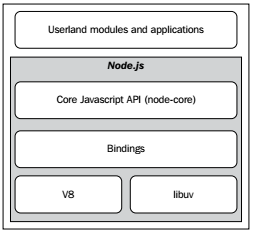
\includegraphics[scale=1.0]{grafiken/nodeArchitecture.png}
     \caption{Node.js architecture \cite{nodejsbook}}
  \end{figure}

\paragraph{Node core}
is a JavaScript library (called node-core) that implements the high-level Node.js API.

\paragraph{Bindings}
responsible for wrapping and exposing libuv and other low-level functionality to JavaScript.\cite{nodejsbook}

\paragraph{Non blocking I/O}
Non blocking I/O in NodeJS is provided by libuv\cite{nodejsabout}\cite{nodejsbook}. 
Which is "a multi-platform support library with a focus on asynchronous I/O. "\cite{libuv} with following properties\cite{libuvBasic}:
\begin{itemize}
\item Abstract operations, not events
\item Support different nonblocking I/O models
\item Focus on embeddability and perfomace
\end{itemize}

\paragraph{V8/Chakra} the JavaScript engine originally developed by Google for the Chrome browser/ Microsoft for IE 9 browser"\cite{nodejsbook} 

\subsection{Event}
"Much of the Node.js core API is built around an idiomatic asynchronous event-driven architecture in which certain kinds of objects (called "emitters") periodically emit named events that cause Function objects ("listeners") to be called.

All objects that emit events are instances of the EventEmitter class. These objects expose an eventEmitter.on() function that allows one or more functions to be attached to named events emitted by the object.

When the EventEmitter object emits an event, all of the Functions attached to that specific event are called synchronously."\cite{events}

\subsection{Event handling}
Node.js  event handler is an implementation of reactor pattern (\ref{fig:nodeEvent}). The description of process lifecycle is shown on Fig. \ref{fig:nodeEvent}:

\begin{figure}[ht]
  	\label{fig:nodeEvent}
    \centering
    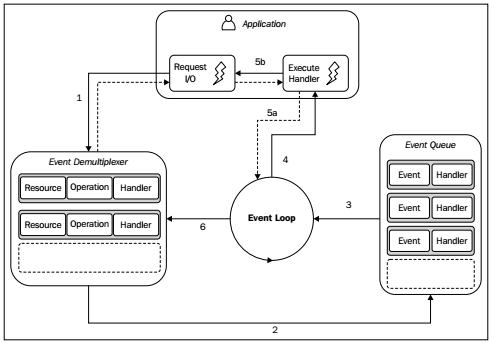
\includegraphics[width=\textwidth]{grafiken/nodeEventHandling.png}
     \caption{Node.js event handling system \cite{nodejsbook}}
  \end{figure}

\begin{enumerate}
\item The application generates a new I/O operation by submitting a request to the Event Demultiplexer. The application also specifies a handler, which will be invoked when the operation completes. Submitting a new request to the Event Demultiplexer is a non-blocking call and it immediately returns the control back to the application.
\item When a set of I/O operations completes, the Event Demultiplexer pushes the new events into the Event Queue.
\item At this point, the Event Loop iterates over the items of the Event Queue.
\item For each event, the associated handler is invoked.
\item The handler, which is part of the application code, will give back the control to the Event Loop when its execution completes. However, new asynchronous operations might be requested during the execution of the handler, causing new operations to be inserted in the Event Demultiplexer, before the control is given back to the Event Loop.
\item When all the items in the Event Queue are processed, the loop will block again on the Event Demultiplexer which will then trigger another cycle.
\end{enumerate}

\section{Asynchronous handling strategies}
\subsection{Callbacks}
Presence of Functions as a first class citizens in javascript allows the usage of functions for handling asynchronous program behavior. Callbacks are handlers for the reactor pattern described before. They are similar to Visitor Pattern in OOP, they also represent an operation to be preformed on the elements of an object structure and it lets you define a new operation without introducing any changes to the definition of the object. 

Callbacks implement continuation-passing-style from FP. By convention callbacks must be passed as the last argument and accept two parameters, the first is an error and the second is a data to be processed further.

There are negative sides of using callbacks. One of them is so called \textit{callback hell} occurs due to the abundance of closures and in-place callback definitions. This makes the code hard to be read because of high level nesting, as well as written due to a scope of nesting and difficult to manage because of possible memory leaks created by closures. Another negative side is called \textit{releasing Zalgo}\cite{zalgo}, it occurs only in case of inconsistent function behavior, when under some hidden conditions a function performs synchronous action but some under other - asynchronous.

\subsection{Data focused strategies / Imperative}
The explanation of asynchronous patterns in this chapter will be performed via mapping of \textit{synchronous} patterns to the \textit{asynchronous}. Another dimension of mapping is \textit{singular} vs \textit{plural}. 

Before starting imperative strategies for handling of asynchronous data flow we would like to show the concept of duality showed by Erik Meijer \url{https://channel9.msdn.com/Events/Lang-NEXT/Lang-NEXT-2014/Keynote-Duality} and hardly used by Kris Koval in his General Theory of Reactivity \url{https://github.com/kriskowal/gtor/}. This chapter is based on works of Kris Koval, Erik Meijer, Conal Eliot and Mark S. Miller in a field of Reactive Programming.\\

During communication can occurred the problem caused by the fact that different parts for the dialog can have different load and different performance, this case is mostly related to asynchronous  case since this parts are distributed. The problem can be divided in to two types of situations.

The first situation is \textbf{Fast producer - slow consumer}. It means that get of one entity works faster then set of next entity in the chain. This situation occurs when values are \textbf{\textit{pushed}} by producer.
The second situation is \textbf{Slow producer - fast consumer}. It means that get of one entity works slower then set of next entity in the chain. This situation occurs when values are \textbf{\textit{pulled}} by consumer. 

Solution of  this problems lays on scope of the system design which should allocate push and pull entities in a appropriate sides of the communication channels.


\paragraph{Value} is a singular unit of \textit{synchronous} data. It has two duals, they are \textit{getter (pull)} and \textit{setter (push)}. Setter accepts value to be assigned and return nothing and getter accepts nothing and returns a value. The chaining process  can be performed here by applying setter to getter and getter to setter and by applying same logic to their analogs for further  entities.

\paragraph{Collection} is \textit{synchronous} and it is a plural form of the value. The duals of a collection are \textit{iterator (pull)} and \textit{generator (push)}. Iterator as a plural analog of getter, it accepts nothing and returns the element from collection. Generator is a plural analog of setter it accepts element to be added to collection and returns nothing.


?! Which of the duals will do blocking ?!


\paragraph{Deferred} is \textit{asynchronous} analog of the value. The duals for promise are \textit{resolver (push)} and \textit{promise (pull)}. The resolver is an asynchronous analog of setter. It  accepts value which will be assigned as soon as it will be resolved. The promise is an asynchronous analog of the getter . It allows to obtain the value of the promise as soon as it will be resolved. The deferred concept guaranties unidirectional data flow which means that data can go in one and the only one direction from resolver to promise. Further deferred entities guaranties asynchronicit execution of am operation which means they are 'Zalgo safe'\cite{asyncPerformance}.

\paragraph{Stream} is \textit{asynchronous} analog of the collection. It can be treated as a collection of deferred elements. The duals for stream are \textit{write (pull)} and \textit{read (push)}. The read is an analog of iterator it accepts nothing and pulls values from the stream.The write is an analog of generator it accepts values from the stream and returns nothing. As a plural analog of deferred it guaranties unidirectional data flow which means that data can go in one and the only one direction from read to write. 
The special case for streams in Node.js are transform and duplex streams which are combination of read and write.

For more information about reactive programming with javascript please visit \url{https://github.com/kriskowal/gtor/}.


The matrix of presented on (Fig. \ref{fig:dualityMatrix}).

\begin{figure}[ht]
  	\label{fig:dualityMatrix}
    \centering
    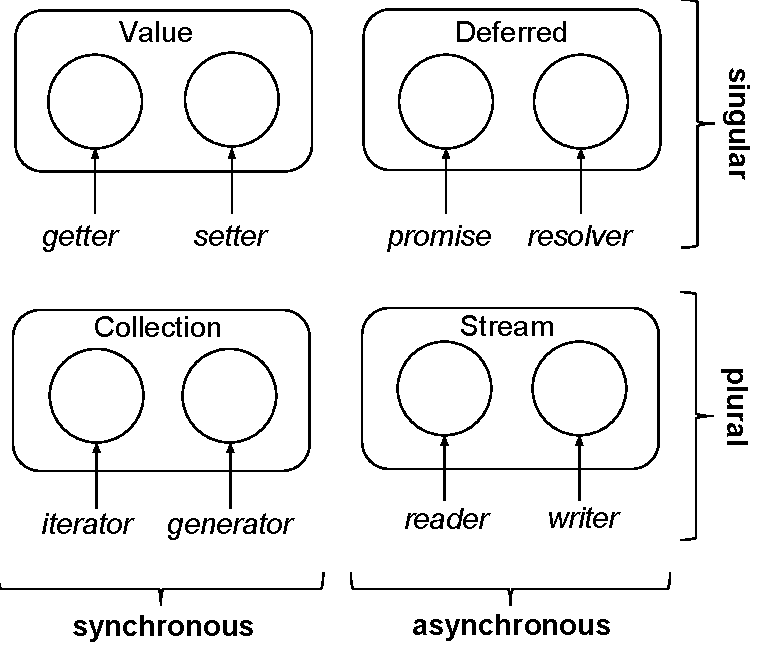
\includegraphics[scale = 0.5]{grafiken/dualityMatrix}
     \caption{Duality Matrix \cite{gtor}}
  \end{figure}
  

%\subsubsection{Streams}
%"A stream is an abstract interface implemented by various objects in Node.js." \cite{nodejsstreams}
%"Dominic Tarr (one of top contributors to the Node.js community \cite{nodejscontributors}), defines streams as node's best and most misunderstood idea."\cite{nodejsbook}

%Streams are the classic example of Pipe-and-filter architecture.

%"In an event-based platform such as Node.js, the most efficient way to handle I/O is in real time, consuming the input as soon as it is available and sending the output as soon as it is produced by the application."\cite{nodejsbook}

%\paragraph{Spatial efficiency.}
%"First of all, streams allow us to do things that would not be possible, by buffering data and processing it all at once. For example, consider the case in which we have to read a very big file, let's say, in the order of hundreds of megabytes or even gigabytes. 
%Clearly, using an API that returns a big buffer when the file is completely read, is not a good idea.
%Imagine reading a few of these big files concurrently; our application will easily run out of memory. Besides that, buffers in V8 (default NodeJS engine) cannot be bigger than 0x3FFFFFFF bytes (a little bit less than 1 GB). 
%So, we might hit a wall way before running out of physical memory." \cite{nodejsbook}

%\paragraph{Time efficiency.}
%"Let's now consider the case of an application that compresses a file and uploads it to a remote HTTP server, which in turn decompresses and saves it on the filesystem.
%If our client was implemented using a buffered API, the upload would start only when the entire file has been read and compressed. On the other hand, the decompression will start on the server only when all the data has been received. 
%A better solution to achieve the same result involves the use of streams. 
%On the client machine, streams allows you to compress and send the data chunks as soon as they are read from the filesystem, whereas, on the server, it allows you to decompress every chunk as soon as it is received from the remote peer."\cite{nodejsbook}

%\paragraph{Composability.}
%"The code we have seen so far has already given us an overview of how streams can be composed, thanks to the pipe() method, which allows us to connect the different processing units, each being responsible for one single functionality in perfect Node.js style. 
%This is possible because streams have a uniform interface, and they can understand each other in terms of API. The only prerequisite is that the next stream in the pipeline has to support the data type produced by the previous stream, which can be either binary, text, or even objects, as we will see later in the chapter.\\
%For these reasons, streams are often used not just to deal with pure I/O, but also as a means to simplify and modularize the code."\cite{nodejsbook}



%\subsection{Piping patterns}
%"As in real-life plumbing, Node.js streams also can be piped together following different patterns; we can, in fact, merge the flow of two different streams into one, split the flow of one stream into two or more pipes, or redirect the flow based on a condition. In this section, we are going to explore the most important plumbing techniques that can be applied to Node.js streams."\cite{nodejsbook}

%\paragraph{Combining streams} - encapsulation of sequentualy connected streams in to single looking stream with single I/O points and single error handling mechanism by pipeing readable stream in to writable stream.\cite{nodejsbook}
%\paragraph{Forking streams} - piping single readable in to multiple writable streams.\cite{nodejsbook}
%\paragraph{Merging streams} - piping multiple readable streams in to single writable stream.\cite{nodejsbook}
%\paragraph{Multiplexing and demultiplexing} - forking and merging pattern which provides shared communication chanel for entities from different sreams.\cite{nodejsbook}
%\cite{nodejsbook}



\section{Performance}
Following measures are taken from the article 'Analysis of generators and other async patterns in node' by Gorgi Kosev (\url{https://spion.github.io/posts/analysis-generators-and-other-async-patterns-node.html}). 

There are no hardware characteristics provided for the experiment execution environment except following: "On my machine redis can be queried about 40 000 times per second; node's "hello world" http server can serve up to 10 000 requests per second; postgresql's pgbench can do 300 mixed or 15 000 select transactions per second." \cite{asyncPerformance_2}

 The performance metrics were taken from the experiment under the following conditions: "All external methods are mocked using setTimeout 10ms to simulate waiting for I/O with 1000 parallel requests (i.e. 100K IO / s) \cite{asyncPerformance_2}

\begin{table}[h]
	\begin{center}
		\begin{tabular}{| l | l | l | }
			\hline
			\textbf{pattern} & \textbf{time(ms)} & \textbf{memory (MB)} \\
			\hline
			promises-bluebird & 512 & 57,45 \\
			\hline
			promises-bluebird-generator & 364 & 41,89 \\
			\hline
			callbacks & 316 & 34.97 \\
			\hline
		\end{tabular}
	\end{center}
	\caption{Performance comparison of patterns for asynchronous information flow \cite{asyncPerformance_2}\cite{asyncPerformance}}
\end{table}


"The original and flattened solutions are the fastest, as they use vanilla callbacks"\cite{asyncPerformance}

Note that this table has only fastest among promise objects and since there were no measurements performed for streams but according to their nature the most optimistic performance for them should be equal to the promise generator.

The mismatch which can occur between results of this experiment and real life lays withing fast producer - slow consumer / slow producer - fast consumer occasion described above.



